\section{Umsetzung}
Das Architekturbild~\ref{fig:umsetzung_frontendarchitektur_4} auf Seite~\pageref{fig:umsetzung_frontendarchitektur_4}
zeigt die Architektur des Frontends und die Kommunikation mit dem API Connect Service. Dabei sollen sowohl das Frontend
als auch die Smartphone-Apps mit dem API Gateway kommunizieren, um die Anfragen zu vereinheitlichen.

Ein Cloud Foundry-Container wird mit einem Node.js-Boilerplate versehen. Mit Hilfe des Boilerplates lassen sich
Node.js-Applikationen innerhalb des Containerts verwalten und nutzen. Es stellt eine Runtime zur Verfügung, in welcher
das Frontend laufen kann.

Die Smartphone-Apps werden auf Basis von Android und auch iOS entwickelt. Beide Systeme erhalten innerhalb der App ein
WebView-Layout, welche für das Laden und das Darstellen der Webseite zuständig ist. Damit ist es einfach, eine schon
erstellte, responsive Webseite optimal für ein Smartphone zu nutzen. Zusätzlich können Feinheiten wie angepasste Layouts
der einzelnen Systeme übernommen werden.

Die Kommunikation zwischen Frontend und API Connect sowie zwischen den entwickelten Smartphone-Apps und dem API Connect
Service laufen über REST-Aufrufe (englisch REST-Calls).

Da in den Smartphone-Apps lediglich das schon geschriebene Frontend geladen wird, müssen die Aufrufe nur ein Mal
spezifiziert und umgesetzt werden.

\begin{figure}[h]
    \centering
    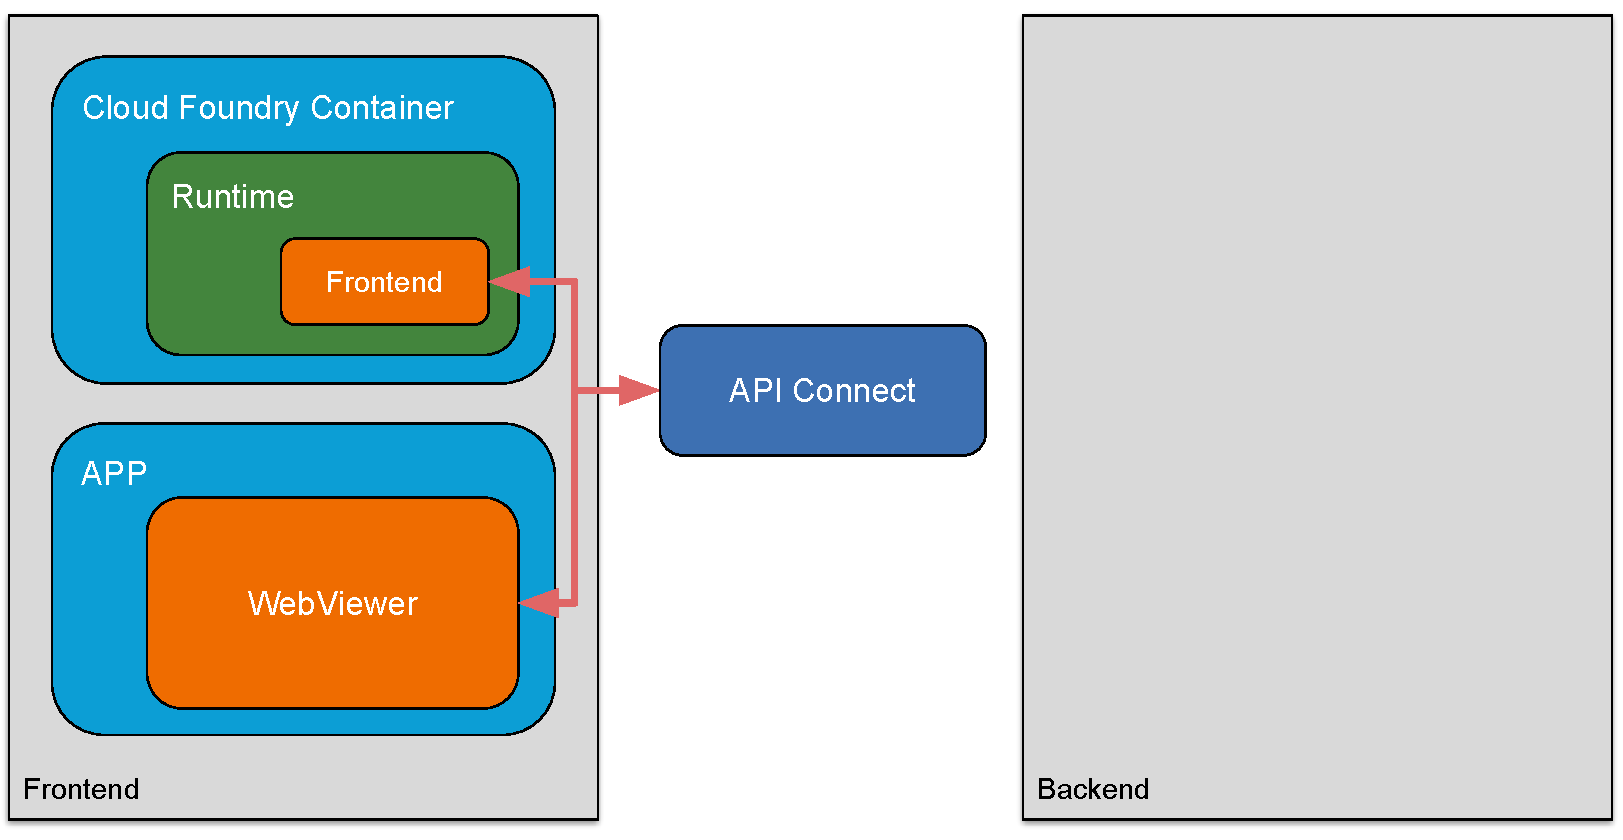
\includegraphics[width=\textwidth]{images/kapitel_4/architektur_frontend.pdf}
    \caption{Übersicht der Zielarchitektur}
    \label{fig:umsetzung_frontendarchitektur_4}
\end{figure}

\subsection{Web-Frontend}
\label{subsec:webseite}
Als nächstes kann man das Web-Frontend (auch Webseite oder englisch website oder auch client genannt) entwickeln. Um
nicht mit zahlreiche Iterationen und Anpassungen bei der Entwicklung zu kämpfen, empfiehlt es sich mit der Definition
von Use-Cases \textendash{} also mit der Definition der Aktionen eines Endnutzers auf der Webseite \textendash{} zu
beginnen.

Anschließend sollte man für die einzelnen Use-Cases Mockups erstellen, die aufzeigen, wie ein Endnutzer die einzelnen
Aktionen durchführen kann. In einem weiteren Schritt setzt der Entwickler die gebauten Mockups dann in Quellcode um,
damit ein Prototyp enstehen kann. Diesen könnte man dann mit einer ausgewählten Gruppe testen.

Damit die Benutzung der Webseite von verschiedenen Endgeräten aus möglich ist, muss man sich im Weiteren gedanken über
das Thema \textit{Responsive} machen. Wie sich die gebaute Webseite also auf den verschiedenen Displaygrößen anpasst.

Nachdem man die Webseite dann fertig entwickelt hat, muss man sie noch in einen Container installieren. Dies ist über
mehrere Varianten möglich. Auch kann man zusätzliche Erweiterungen einbauen, welche das Arbeiten mit der Webseite
erleichtern oder speziellen Bedürfnissen der Endanwender gerecht wird.

\subsubsection{Use-Cases}
Als Use-Case kommt zum jetzigen Zeitpunkt lediglich eine Aktion in Frage. Das Erstellen von Vorhersagen für die
manuell eingetragenen Parameter der Maschine.

Da das Backend mit seinem neuronalen Netz aktuell nicht mehr berechnen kann, ist der angegebene Use-Case auch der einzig
sinnvolle.

Nachdem der Endnutzer die Parameter dann in das Formular eingetragen hat, soll er die Möglichkeit bekommen, die
resultierenden Vorhersagen zu erhalten, um diese an der Maschine zu testen. Eine Fortschrittsanzeige soll darüber
informieren, dass das System arbeitet.

Da der Use-Case relativ einfach definiert werden konnte, kann man als nächstes mit der Erstellung der Mockups beginnen,
um eine erste Idee der Anwendung und ihrem Aussehen zu bekommen.

\subsubsection{Mockups erstellen}
Da der Use-Case nun definiert ist, kann man mit der Entwicklung der Mockups beginnen. Dabei ist die Wahl des Designs auf
eine zweispaltige Startseite gefallen. Eine der beiden Spalten beinhlatet die Eingabewerte und die andere Spalte
beinhaltet die vorhergesagten Argumente, welche von dem neuronalen Netz bestimmt werden.

In Abbildung~~\ref{fig:umsetzung_mockup_scale_1} auf Seite~\pageref{fig:umsetzung_mockup_scale_1} zeigt eine erste
Version des Frontends zur Umsetzung der beiden Spalten. Dabei werden in der linken Spalte die Werte in Formularfelder
eingetragen und in der rechten Spalte die vorhergesagten Parameter angezeigt.

Im mittleren Bereich der Seite soll ein Button erscheinen, welcher durch betätigen die eingetragenen Parameter an das
Backend schickt und anschließend den Output anzeigt.

\begin{figure}[h]
    \centering
    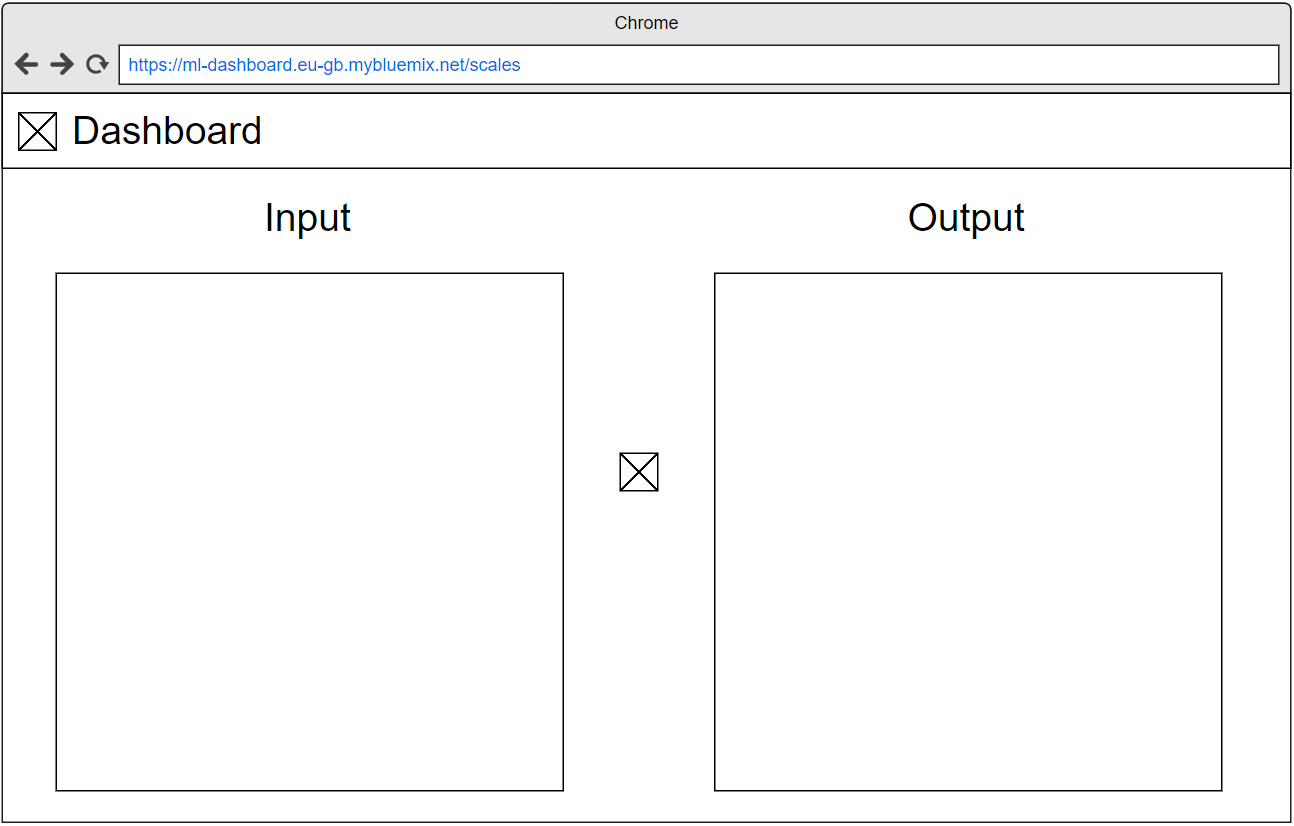
\includegraphics[width=\textwidth]{images/kapitel_4/mockup_scale_1.png}
    \caption{Erstes Mockup für das Dashboard}
    \label{fig:umsetzung_mockup_scale_1}
\end{figure}

Damit man sowohl der Input als auch der Output verbessert anzeigen kann ist es sinnvoll, die beiden Spalten noch weiter
zu unterteilen. Gerade bei den Eingabewerten gibt es zahlreiche Parameter, die in Gruppen zusammengefügt werden können.

So ist es zum Beispiel möglich die Parameter \textit{Produktbreite}, \textit{Produkthöhe} und \textit{Produkttiefe} zu
einer Gruppe namens \textit{Produktmaße} zusammenzufügen.

Die Abbildung~\ref{fig:umsetzung_mockup_scale_2} auf Seite~\pageref{fig:umsetzung_mockup_scale_2} zeigt das angepasste
Mockup mit seinen Gruppen sowohl auf der Input- als auch der Output-Seite.

\begin{figure}[h]
    \centering
    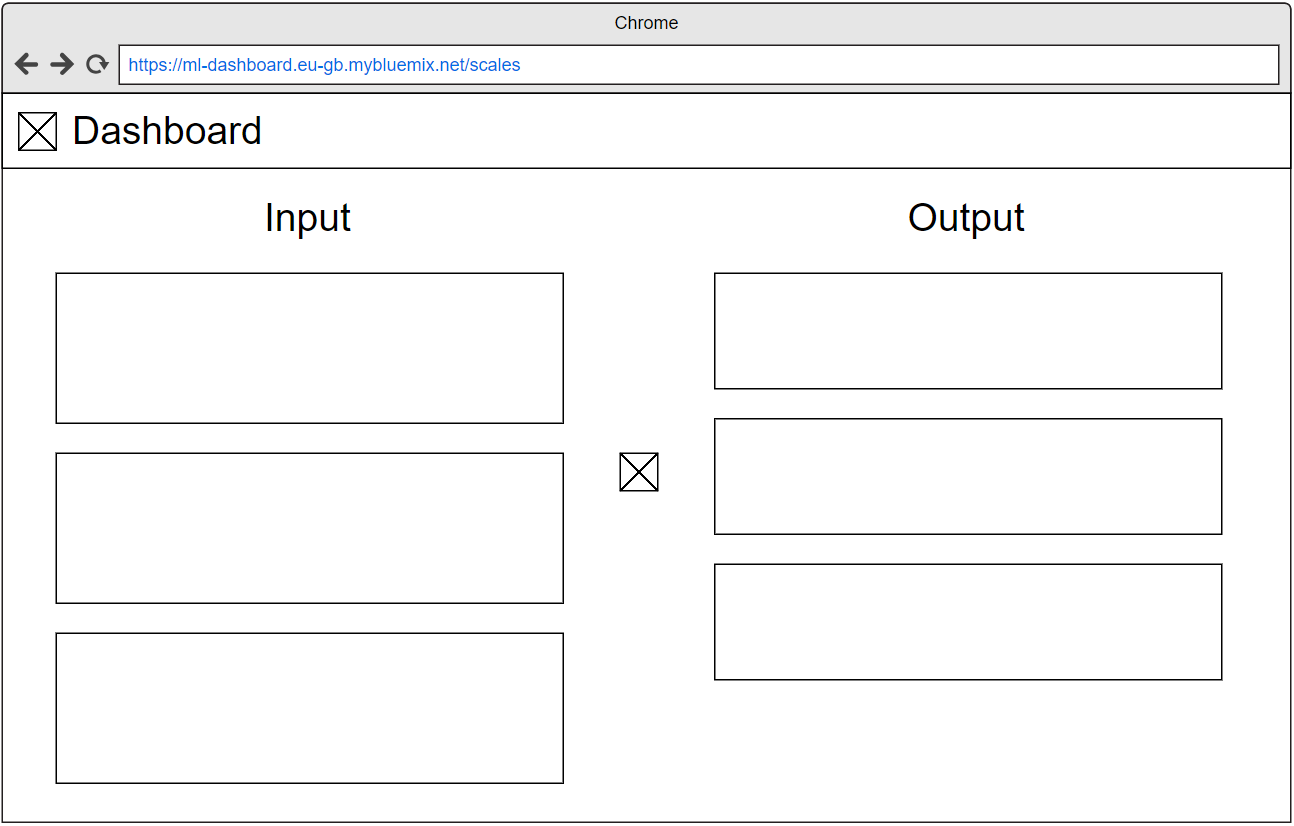
\includegraphics[width=\textwidth]{images/kapitel_4/mockup_scale_2.png}
    \caption{Überarbeitetes Mockup für das Dashboard}
    \label{fig:umsetzung_mockup_scale_2}
\end{figure}

Im oberen Bereich der Anwendung kann man ein Logo der Anwendung erscheinen lassen und nebenan den Namen für die aktuell
geöffnete Seite.

Damit man das Frontend auch für weitere Maschinen oder Maschinenkomponenten anpassen kann, kann der Entwickler ein Menü
hinzufügen, über das man auf die anderen Seiten mit Eingabe- und Ausgabewerte zugreifen kann.

Dieses Menü entwickelt man am Besten so, dass es sich aus dem linken Bereich herausschiebt und über ein
\textit{Hamburger-Menü-Icon}\footnote{https://de.wikipedia.org/wiki/Hamburger-Menü-Icon} zu öffnen ist.

So ist in Abbildung~\ref{fig:umsetzung_mockup_scale_menu} auf Seite~\pageref{fig:umsetzung_mockup_scale_menu} das Mockup
für ein seitliches Menü zu sehen, welches über drei beispielhafte Menüeinträge verfügt.

Das Menü soll sich beim aufklappen über den Inhalt legen und den restlichen Bildschirm etwas ausgrauen, sodass für den
Nutzer ersichtlich ist, dass aktuell am Menü eine Auswahl getroffen werden muss.

Ein Klick in den ausgegrauten Bereich, oder auch auf einen der Menüpunkte, schließt das Menü allerdings wieder, sodass
der Nutzer immer das tun kann, was er gerade möchte.

Die Auswahl eines neuen Menüpunktes hat außerdem zur Folge, dass sich die vorher angesprochene Überschrift im oberen
Bereich der Webseite mit dem Namen des Menüpunktes füllt, damit der Nutzer immer genau weiß, unter welchem Menüpunkt
er sich aktuell befindet.

\begin{figure}[h]
    \centering
    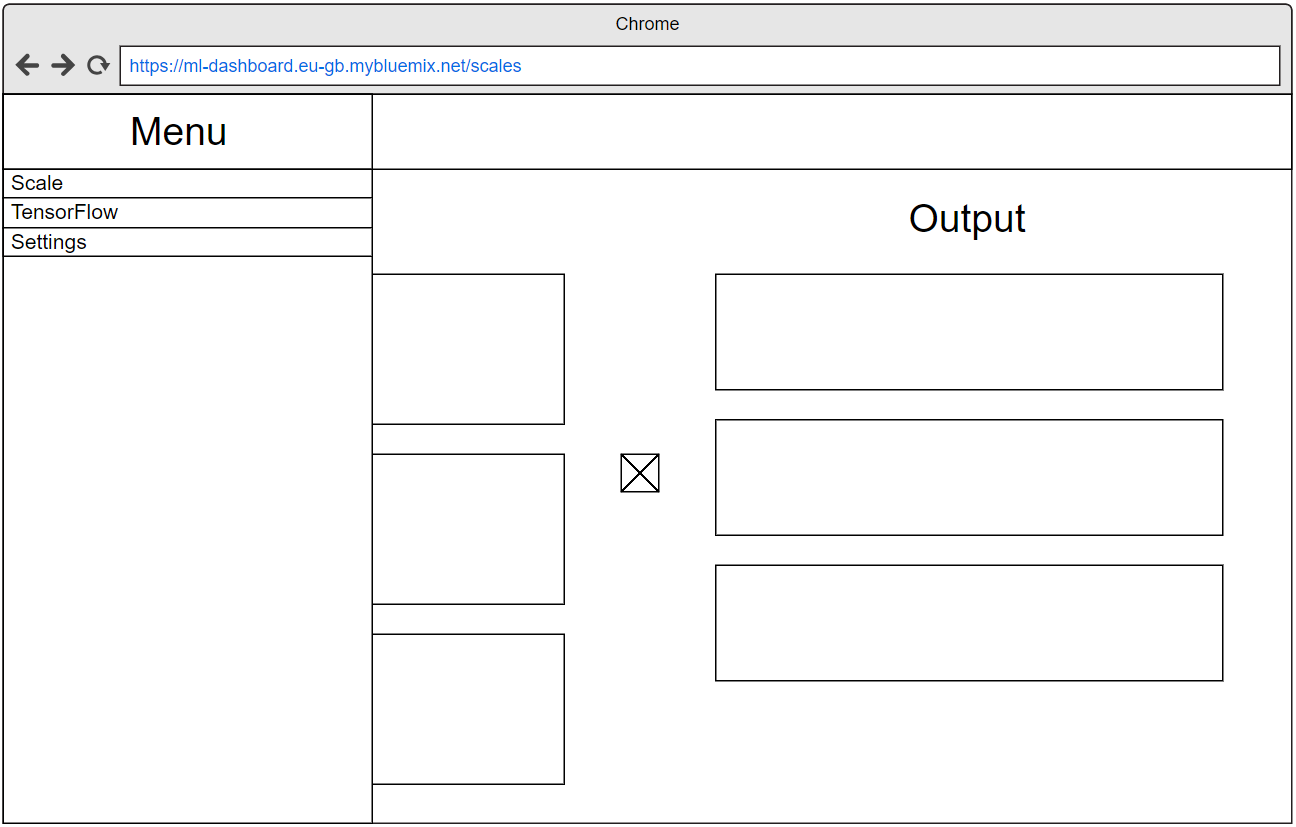
\includegraphics[width=\textwidth]{images/kapitel_4/mockup_scale_menu.png}
    \caption{Mockup für die Navigation}
    \label{fig:umsetzung_mockup_scale_menu}
\end{figure}

\subsubsection{Gedanken zu Responsive}
Damit das Frontend auch von einem Smartphone aus bedient und eine WebView-App dafür geschrieben werden kann, muss die
Webseite auf verschiedene Displaygrößen so reagieren können, damit es alle Informationen nutzerfreundlich anzeigt. Dabei
dürfen keine wichtigen Informationen verschwinden oder die Interaktion mit dem System eingeschränkt sein.

Um dieser Anforderung gerecht zu werden, muss das Frontend mit responsiven Eigenschaften versehen werden. Da die
Webseite in Ihrer ursprünglichen Idee zwei Spalten hat, ist es für die responsive Version interessant, die Spalten nicht
nebeneinander anzuzeigen, sondern untereinander. Dies aber auch nur, sofern es nicht genügend Platz hat, um beide
Spalten nebeneinander anzuzeigen.

Bei größeren Displays wäre es im horizontalen Modus (englisch landscape mode) möglich, beide Spalten auch nebeneinander
anzuzeigen. Wohingegen im vertikalen Modus (englisch portrait mode) immer Sinnvoll ist, die beiden Spalten untereinander
anzuzeigen.

Das Mockup in Abbildung~\ref{fig:umsetzung_mockup_scale_responsive} auf Seite~\pageref{fig:umsetzung_mockup_scale_responsive}
zeigt die Darstellung des Frontends auf einem Smartphone im vertikalen Modus. Dabei ist die Spalte mit der
\textit{Eingabe} aktuell sichtbar und unterhalb wird der Button für die Berechnung der Ausgabeparameter angezeigt.

Unter dem Button ist die Spalte für die Ausgabeparameter angesiedelt, welche erst erscheint, wenn Vorhersagen zur
Verfügung stehen. So ist der Scrollbalken auf der Webseite nicht unnötig lang um den Endnutzer nicht zu verunsichern.

Auch wird nach der Bestätigung des Buttons automatisch zum Bereich der Ausgabe gescrollt, damit dies nicht manuell
geschehen muss.

\begin{figure}[h]
    \centering
    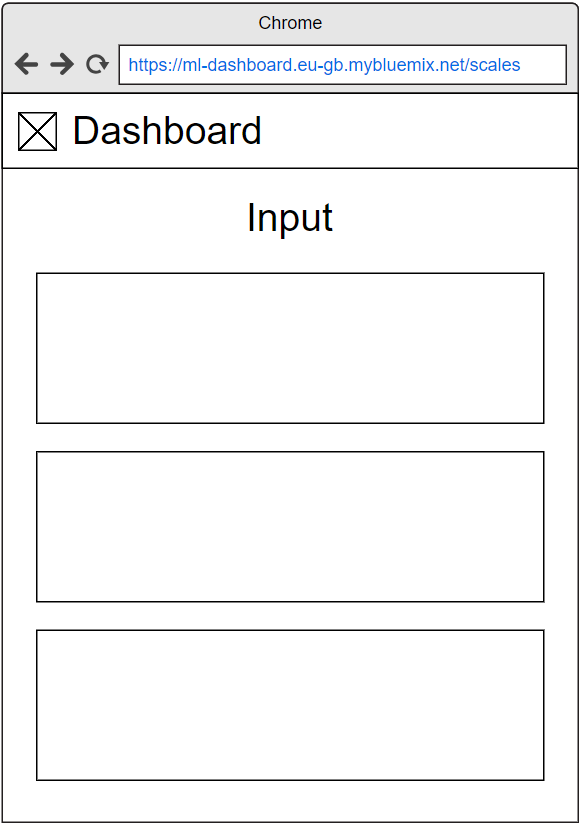
\includegraphics[scale=0.45]{images/kapitel_4/mockup_scale_responsive.png}
    \caption{Mockup des responsiven Designs}
    \label{fig:umsetzung_mockup_scale_responsive}
\end{figure}

\subsubsection{Webseite umsetzen}
Da die Mockups für die Anwendung fertig umgesetzt sind, kann im Weitern damit begonnen werden, das Frontend wirklich
umzusetzen. Da man das Frontend mit Angular umsetzt und die Angular-CLI installiert ist, kann man auf dem
Entwicklerrechner mit dem folgenden Befehl eine neue Angular-Seite einrichten.

\begin{lstlisting}[language=bash, caption=Einrichten einer neuen Angular-Seite, label=ls:umsetzung_angular]
    ng new dashboard
\end{lstlisting}

Dabei wird ein neuer Ordner mit dem Namen \textit{dashboard} angelegt, welcher alle benötigten Ordner und Dateien um
eine funktionierende Angular-Seite zu bauen beinhaltet. Wenn man anschließend in den neu erstellen Ordner wechselt, kann
man mit dem folgenden Befehl die Standard-Applikation von Angular bauen lassen und sie im Browser ansehen.

\begin{lstlisting}[language=bash, caption=Bereitstellen der Angular-Webseite, label=ls:umsetzung_angularserve]
    ng serve --open
\end{lstlisting}

Der Browser öffnet sich automatisch und zeigt die Standardanwendung. Darin ist ein großes Bild des Angular-Logos mit
einer großen Überschrift und ein paar weiteren Kommentaren zu sehen.

Jegliche Änderung am Quellcode der aktuellen Anwendung hat zur Folge, dass die entsprechende Angular-Komponente neu
gebaut und der Browser neu geladen wird um die Änderung direkt sichtbar zu machen.

Nun kann damit begonnen werden, die Webseite entsprechend der Mockups umzusetzen. Dabei ist darauf zu achten, die
Standard-Komponenten der Angular-Material-Bibliothek zu nutzen, damit das Erscheinungsbild der Anwendung einer Android-
App ähnelt.

Die Komponenten sind auf der entsprechenden Dokumentationsseite\footnote{https://material.angular.io/components/categories}
einsehbar und können von da auch direkt kopiert werden um sie im eigenen Quellcode direkt zu nutzen. Auch Icons und
vorgefertigte Farben kann man der Webseite entnehmen um eine im Stil passende Webseite zu bauen.

In Abbildung~\ref{fig:umsetzung_website_input} auf Seite~\pageref{fig:umsetzung_website_input} ist die fertige
umgesetzte Webseite zu sehen, welche die Parameter für das neuronale Netz eingeben kann. Die linke Spalte mit der
\textit{Eingabe} ist also umgesetzt.

\begin{figure}[h]
    \centering
    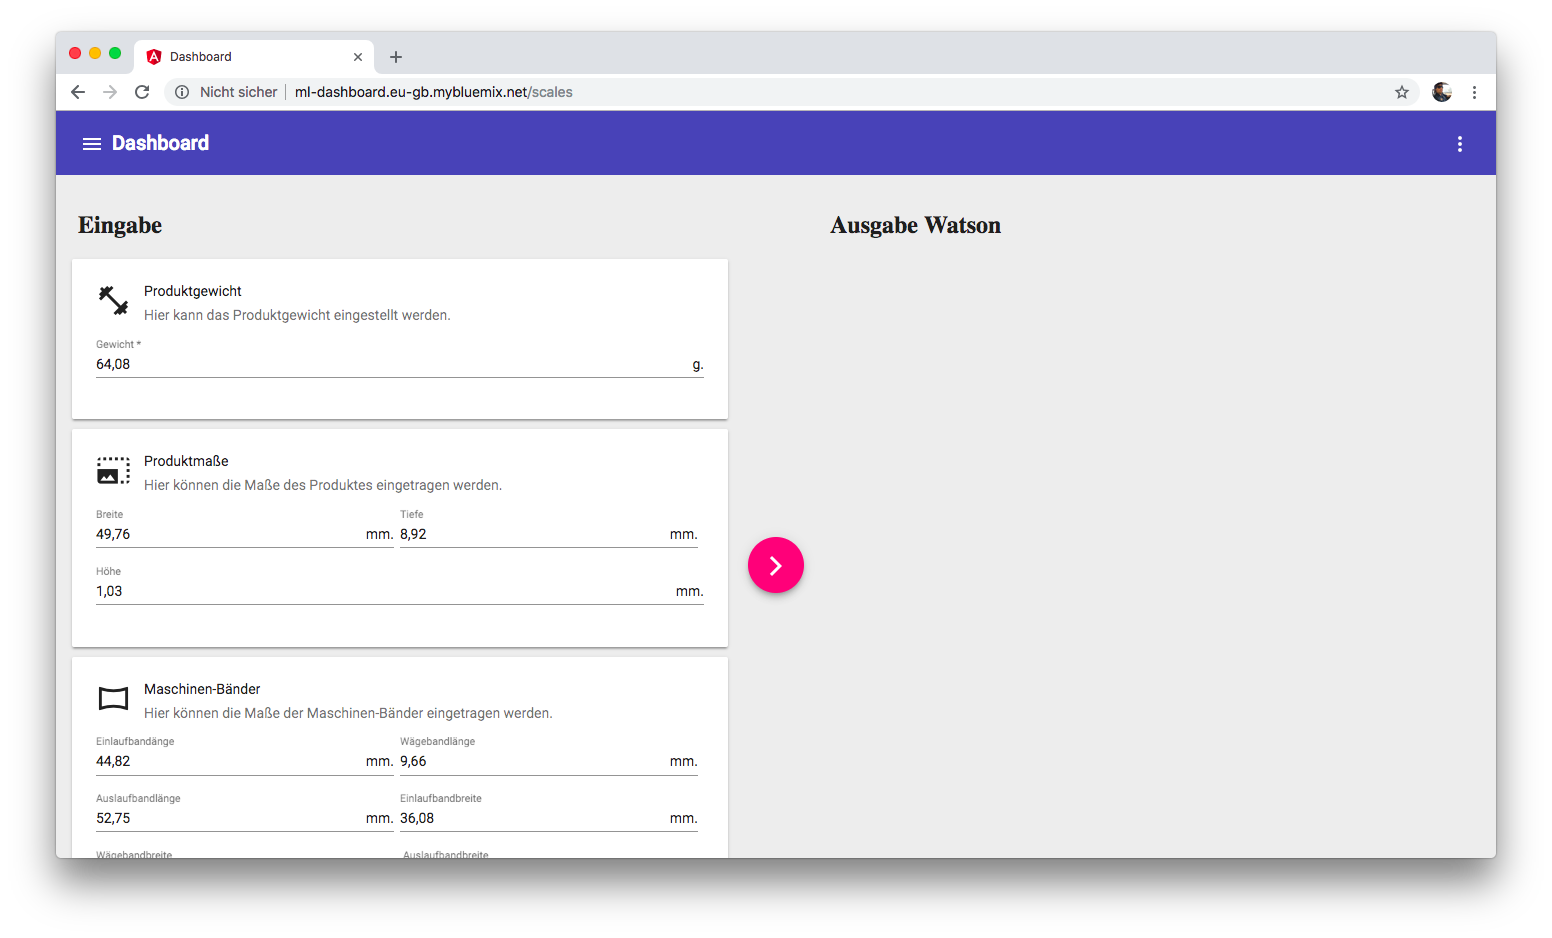
\includegraphics[width=\textwidth]{images/kapitel_4/website_input.png}
    \caption{Umsetzung der Webseite mit Eingabe-Spalte}
    \label{fig:umsetzung_website_input}
\end{figure}

Nun kann man die zweite Spalte mit der \textit{Ausgabe} anfertigen um sie in dem noch leeren Platz zu positionieren. Die
Umsetzung ist dabei gleich der Umsetzung mit der linken Spalte.

In der Abbildung~\ref{fig:umsetzung_website_output} auf Seite~\pageref{fig:umsetzung_website_output} ist die komplette
Webseite zu sehen mit beiden Spalten und dem Button zur generierung der Vorhersage.

\begin{figure}[h]
    \centering
    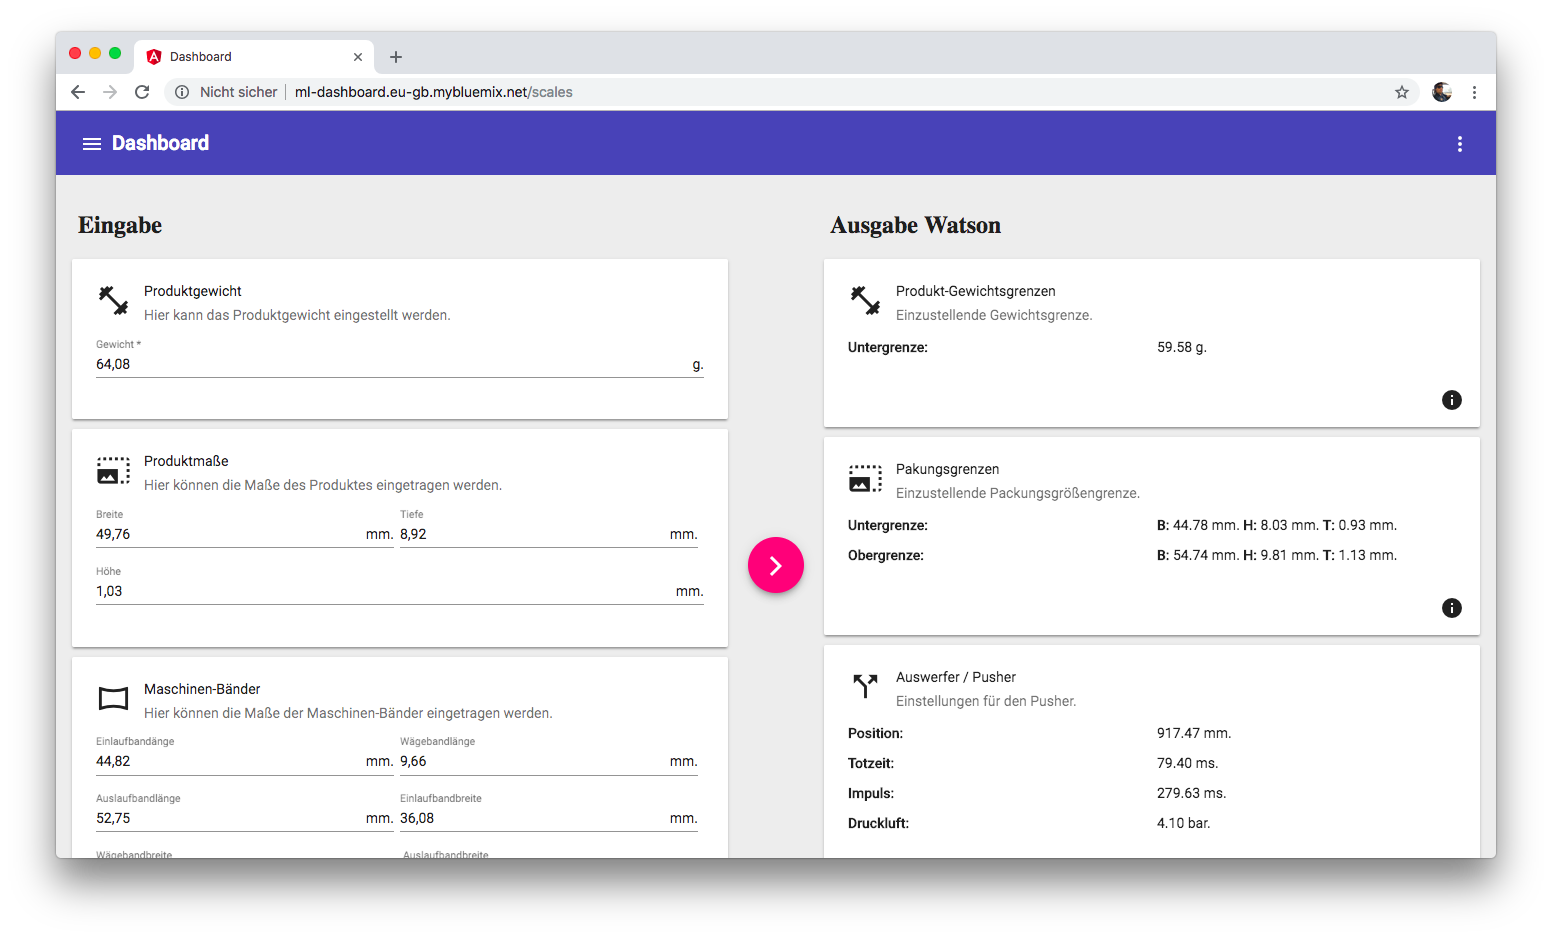
\includegraphics[width=\textwidth]{images/kapitel_4/website_output.png}
    \caption{Umsetzung der Webseite mit Ausgabe-Spalte}
    \label{fig:umsetzung_website_output}
\end{figure}

Bei der Umsetzung ist entscheidend, dass die rechte Spalte des Dashboards nur dann angezeigt wird, wenn auch die Abfrage
an das Backend durch ist und Vorhersagen an das Frontend zurück gekommen sind.

Dies erleichtert die Arbeit mit der Webseite enorm, da der Endnutzer nicht direkt mit vielen Boxen konfrontiert wird.
Außerdem existieren für die rechte Spalte nach dem öffnen der Seite auch noch keine Daten die angezeigt werden könnten.
So macht eine Darstellung des Bereiches auch keinen Sinn.

Damit der Endnutzer sich schneller auf der Webseite zurecht finden kann, ist die Platzierung von kleinen Icons und
Beschreibungstexten an den verschiedenen Boxen sinnvoll. So weiß der Nutzer direkt, was er in welcher Box machen oder
auch Einstellen kann.

Sinnvoll ist es auch die Parameter der linken Spalte mit passenden Zufallszahlen zu versehen. So kann der Nutzer direkt
nach dem öffnen der Seite eine Vorhersage starten um die Funktionsfähigkeit der Webseite und des Backends zu testen.
Auch kann er so nachvollziehen, welche Werte er in der linken Spalte eintragen muss, falls er sich zuanfang noch
unsicher ist.

Als nächsten Schritt muss man die Anpassung der Webseite an einen kleineren Bildschirm machen. Die Darstellung kann den
Mockups entnommen werden. Da die beiden Spalten (Eingabe und Ausgabe) in jeweils einer eigenen Angular-Komponente
entwickelt sind, kann man diese in eine \textit{CSS-FlexBox} packen.

Damit ist es möglich zu definieren, wie sich die einzelnen \textit{FelxBoxen} verhalten, wenn der Platz nicht
ausreichend ist. Dabei gibt man an, dass die Boxen sich im normalen Fall nebeneinander befinden. Falls dann der Platz
nicht ausreicht, sollen sie sich untereinander anordnen.

Dabei ist wichtig, dass der Button in der Mitte auch eine FlexBox erhält, damit dieser bei kleinem Platz auch
umgebrochen werden kann. Die Umbrechnung übernimmt die Bibliothek automatisch und es bedarf keiner weiteren
Konfiguration.

Ein Test mit einem mobilen Browser oder den Dev-Tools des Explorers \textit{Chrome} oder auch \textit{FireFox} zeigt die
Abbildung~\ref{fig:umsetzung_website_smartphone} auf Seite~\pageref{fig:umsetzung_website_smartphone}. Es ist lediglich
die \textit{Eingabe}-Spalte zu sehen.

\begin{figure}[h]
    \centering
    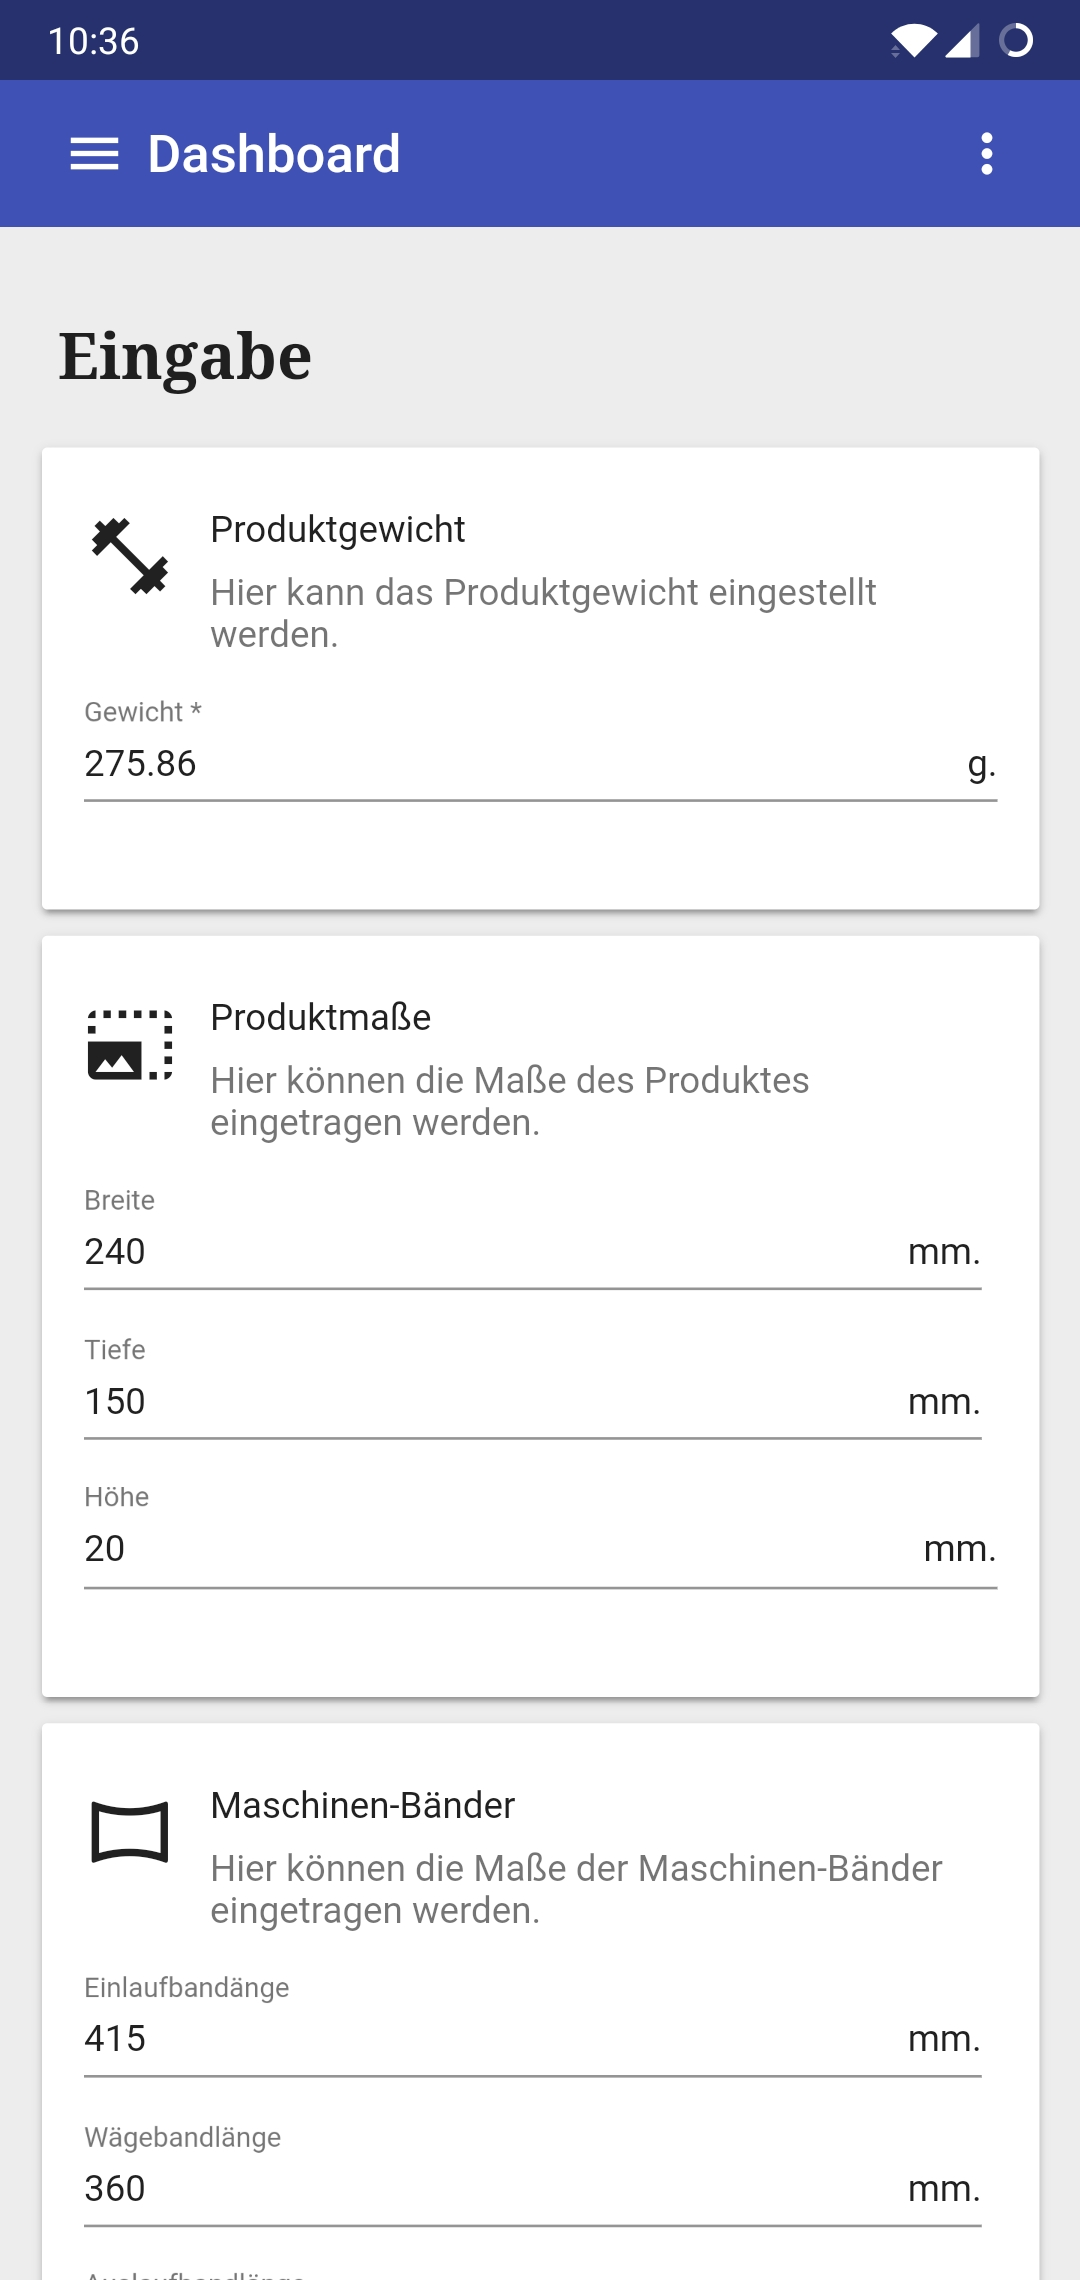
\includegraphics[scale=0.13]{images/kapitel_4/website_smartphone.jpg}
    \caption{Umsetzung der Webseite mit responiven Fähigkeiten}
    \label{fig:umsetzung_website_smartphone}
\end{figure}

Bei der Eingabe der einzlenen Formularfelder scrollt man unweigerlich nach unten. Am Ende der Eingabe erscheint dann der
Button zum erstellen der Vorhersage für die Parameter.

Nach einem Klick auf diesen Button und einer kurzen Ladeanimation erscheint die Ansicht der Ausgabe. Der Nutzer muss
nicht mehr nach unten scrollen.

%% TODO noch schreiben
\subsubsection{Service Worker}
Die Webseite ist fertig entwickelt. Nun kann man sich über Erweiterungen Gedanken machen, die den Endnutzer bei der
Eingabe unterstützen können.

\colorbox{yellow}{Hier fehlt was}

%% TODO noch schreiben
\subsubsection{Offline Mode}
Dann kann man alles speichern, damit es offline verfügbar ist.
\colorbox{yellow}{Hier fehlt was}

%% TODO noch schreiben
\subsubsection{Weitere Funktionalitäten}
Offline Modus -> Kein Request an API,
\colorbox{yellow}{Hier fehlt was}

%% TODO noch schreiben
\subsubsection{Toolchain einrichten}
\colorbox{yellow}{Hier fehlt was}

\begin{figure}[h]
    \centering
    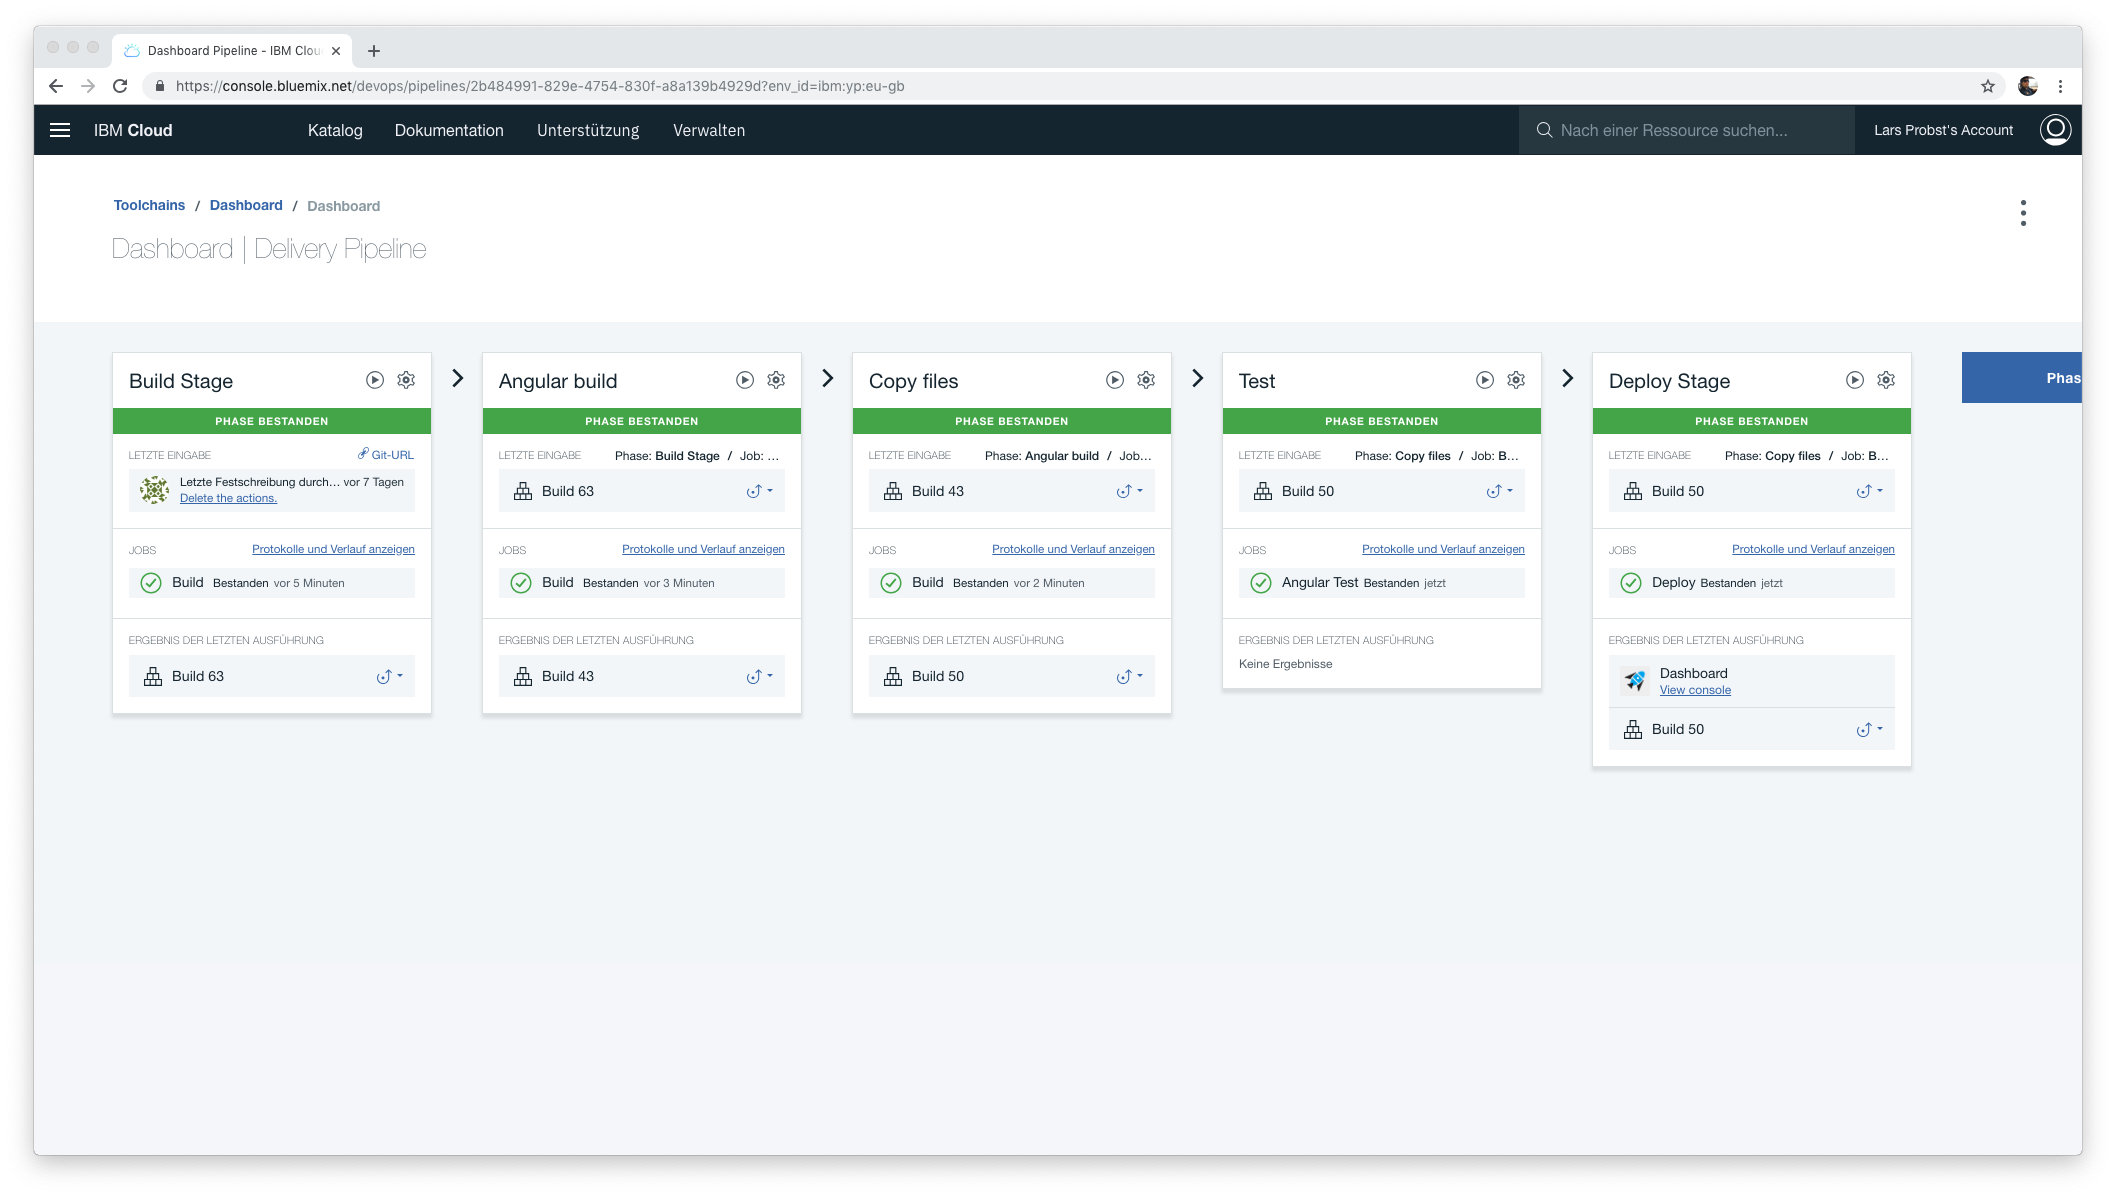
\includegraphics[width=\textwidth]{images/kapitel_4/toolchain_pipeline.png}
    \caption{Übersicht der Toolchain-Konfiguration}
    \label{fig:umsetzung_toolchain_pipeline_frontend}
\end{figure}

\subsection{Smartphone App}
Da das Frontend (Dashboard) nun fertig entwickelt ist, kann man es im nächsten Schritt für die Umsetzung der
Smartphone-App nutzen.

Die Umsetzung der Smartphone-App erfolgt auf Basis von Android und iOS. Dies hat den Vorteil, dass ein größerer
potentieller Kundenkreis gewonnen werden kann, da diese beiden Systeme die mobilen Betriebssysteme
dominieren~\cite{online_umsetzung_mobileos}.

In den zwei weiteren Kapiteln werden die Umsetzungen für die beiden Betriebssysteme erläutert. Insbesondere wird auf die
technischen Unterschiede der Systeme eingegangen.

%% TODO noch schreiben
\subsubsection{Android}
Bauen und erstellen der Apps

\colorbox{yellow}{Hier fehlt was}

\begin{figure}[h]
    \centering
    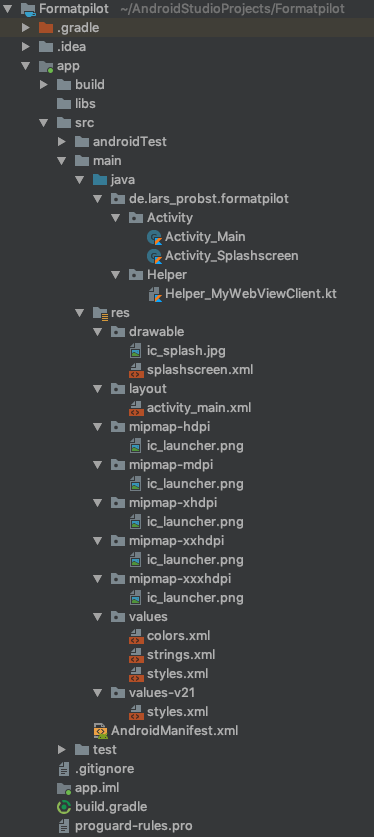
\includegraphics[scale=0.4]{images/kapitel_4/android_folder.png}
    \caption{Ordner und Dateien in Android Studio}
    \label{fig:umsetzung_android_folder}
\end{figure}

\begin{figure}[h]
    \centering
    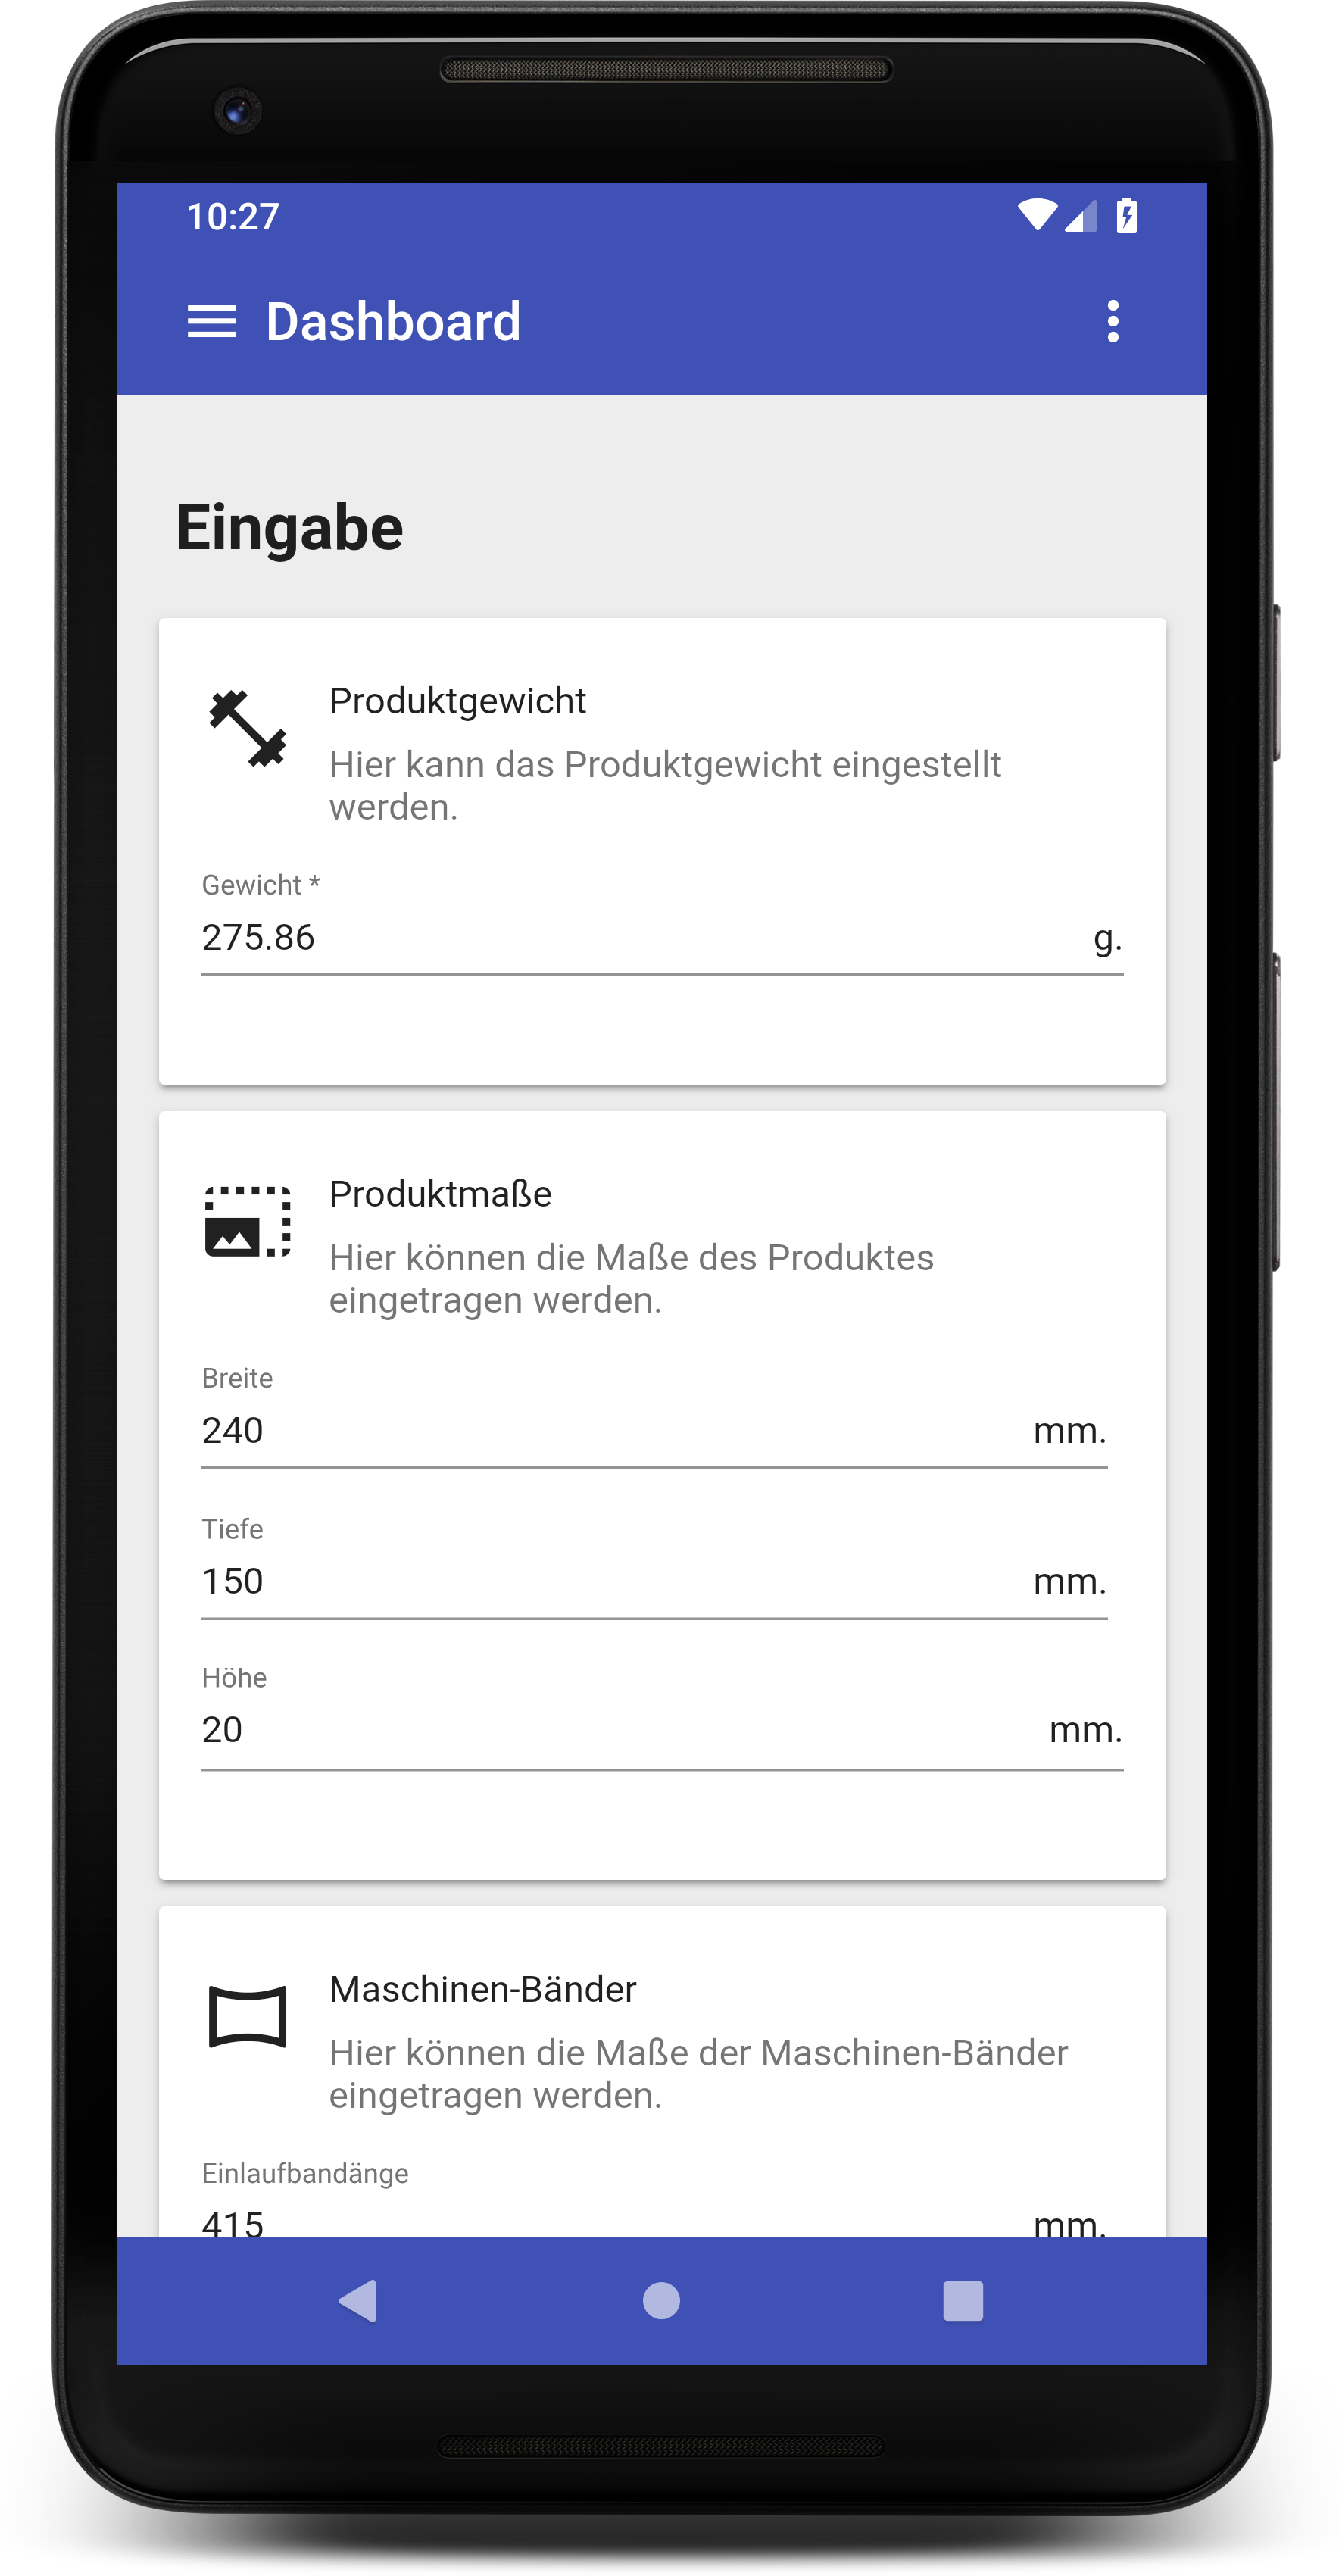
\includegraphics[scale=0.1]{images/kapitel_4/android_app.png}
    \caption{Android-App im Smartphone-Emulator}
    \label{fig:umsetzung_android_app}
\end{figure}

%% TODO noch schreiben
\subsubsection{iOS}
Bauen und erstellen der Apps

\colorbox{yellow}{Hier fehlt was}

\begin{figure}[h]
    \centering
    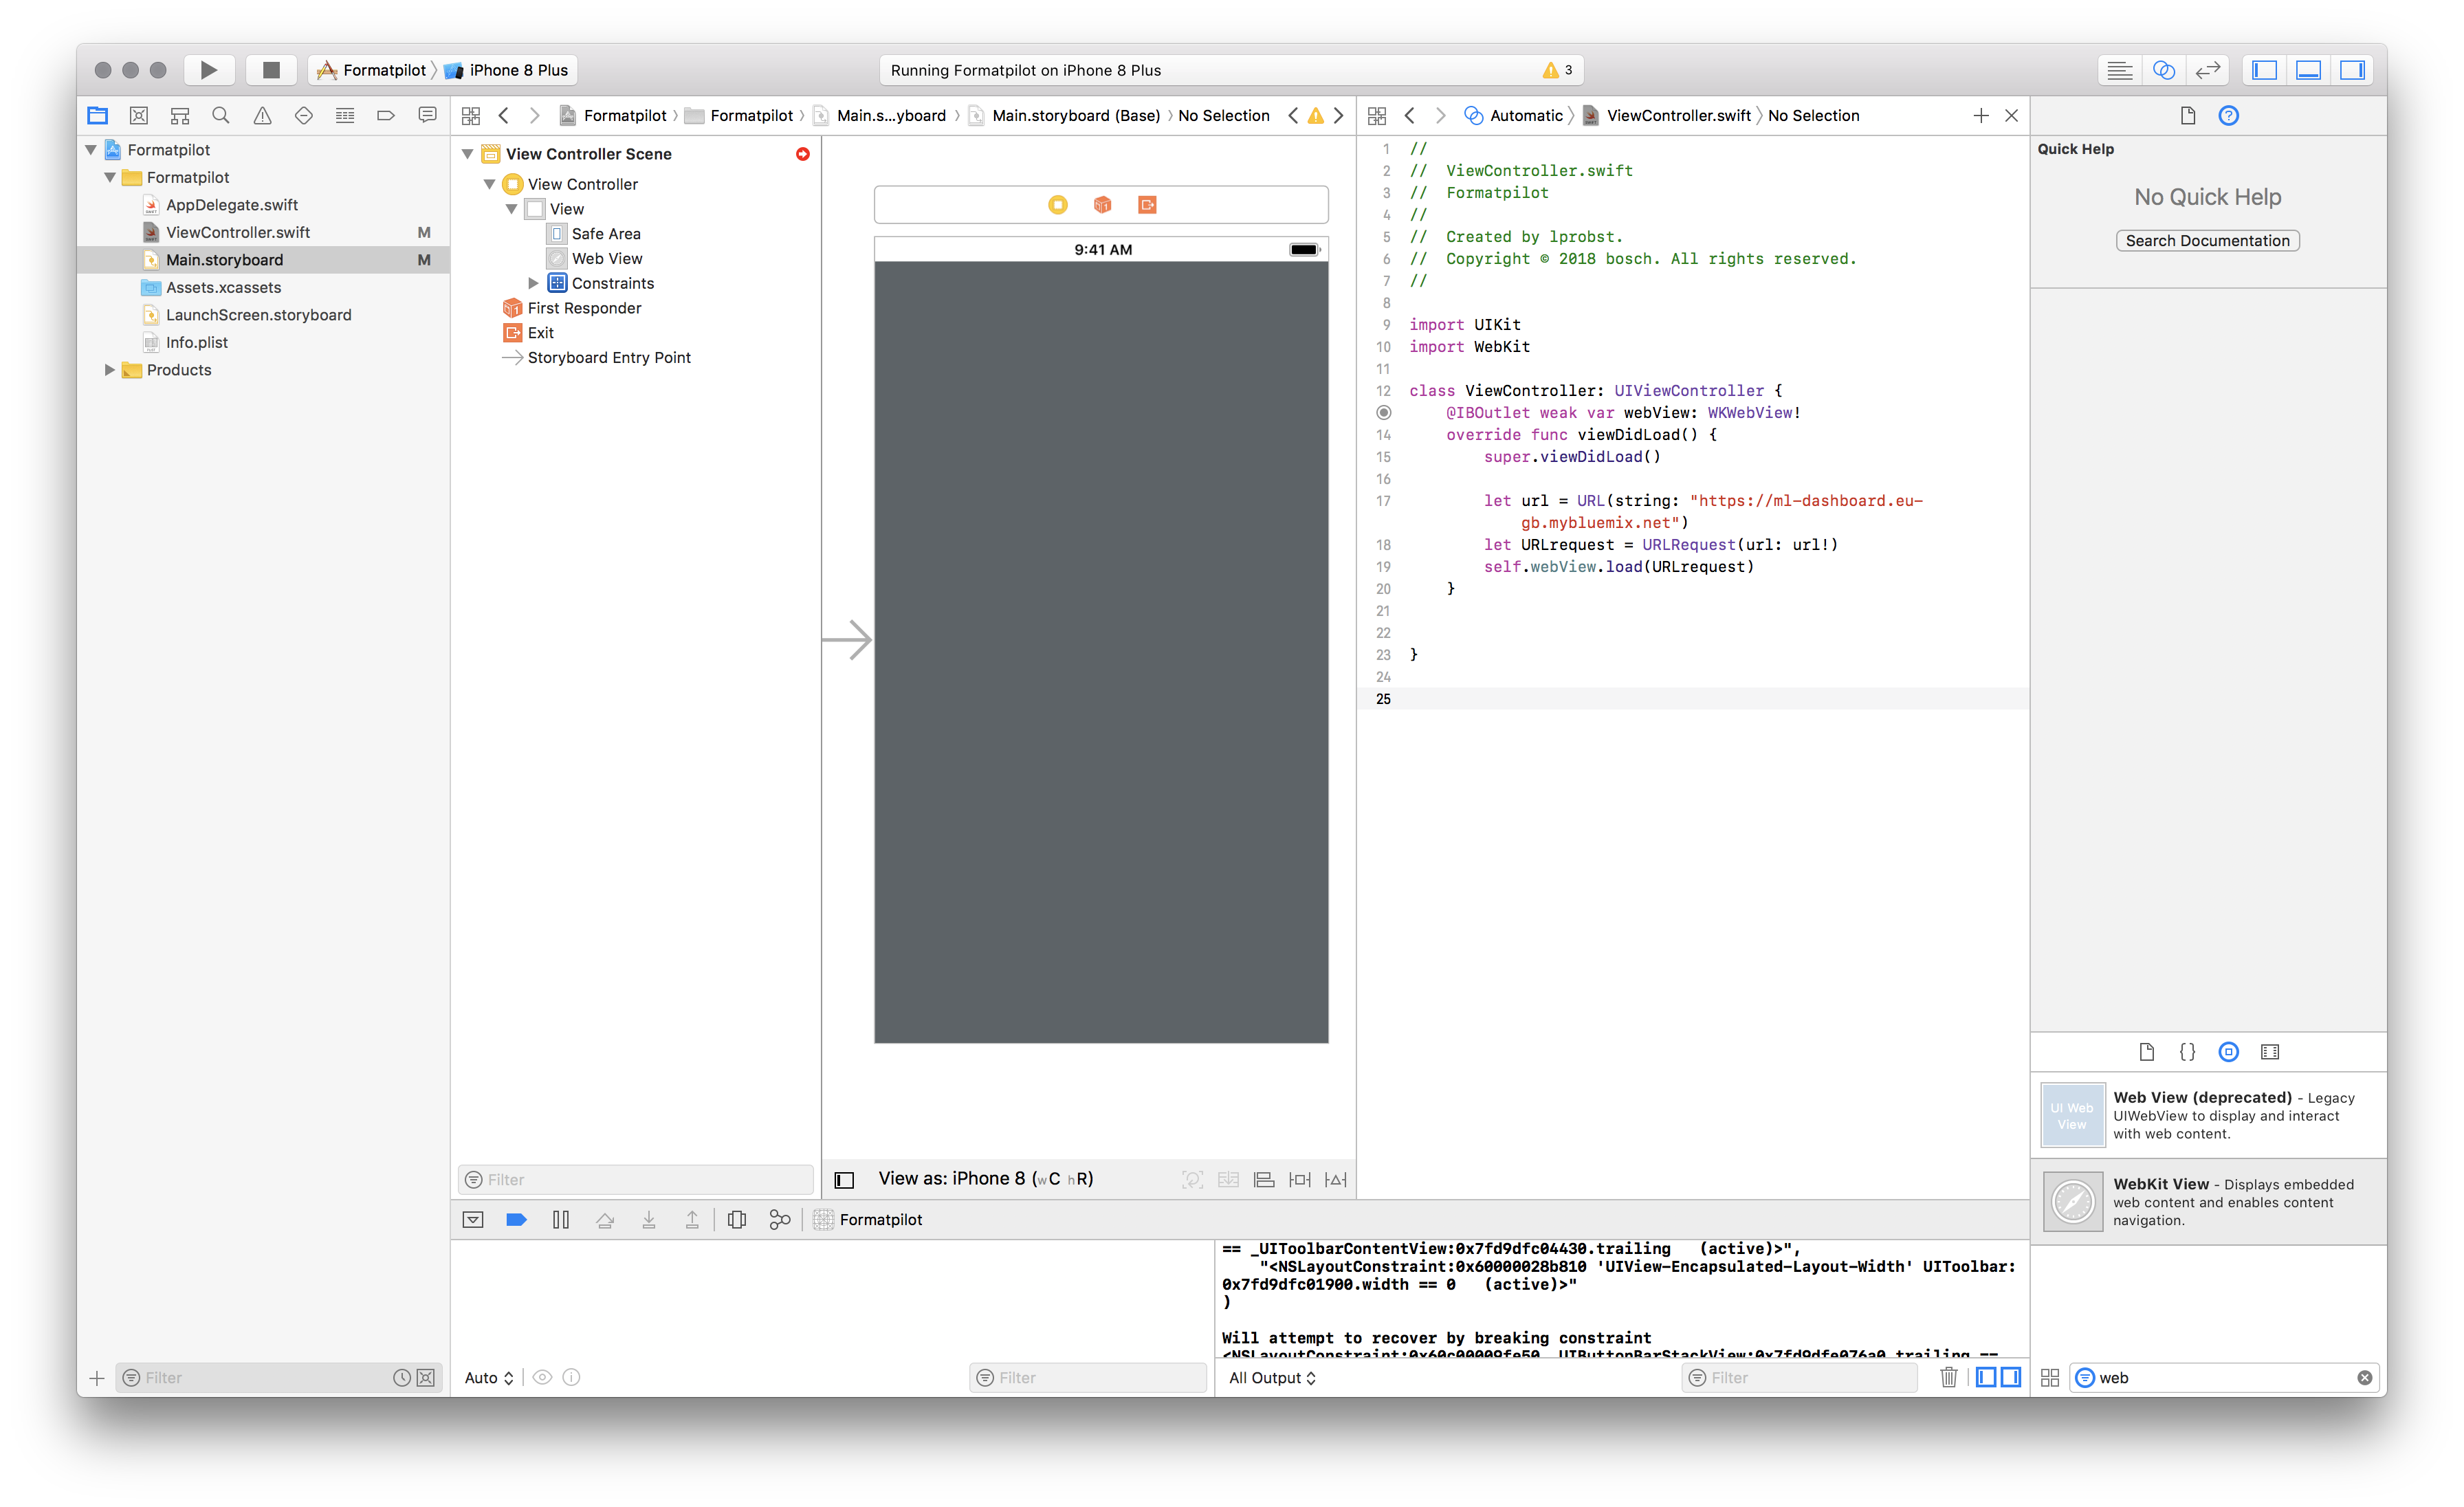
\includegraphics[width=\textwidth]{images/kapitel_4/ios_ide.png}
    \caption{Übersicht von xCode}
    \label{fig:umsetzung_ios_ide}
\end{figure}

\begin{figure}[h]
    \centering
    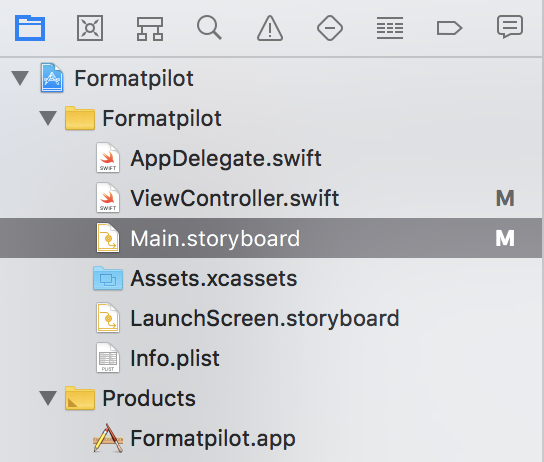
\includegraphics[scale=0.7]{images/kapitel_4/ios_folder.png}
    \caption{Ordner und Dateien in xCode}
    \label{fig:umsetzung_ios_folder}
\end{figure}

\begin{figure}[h]
    \centering
    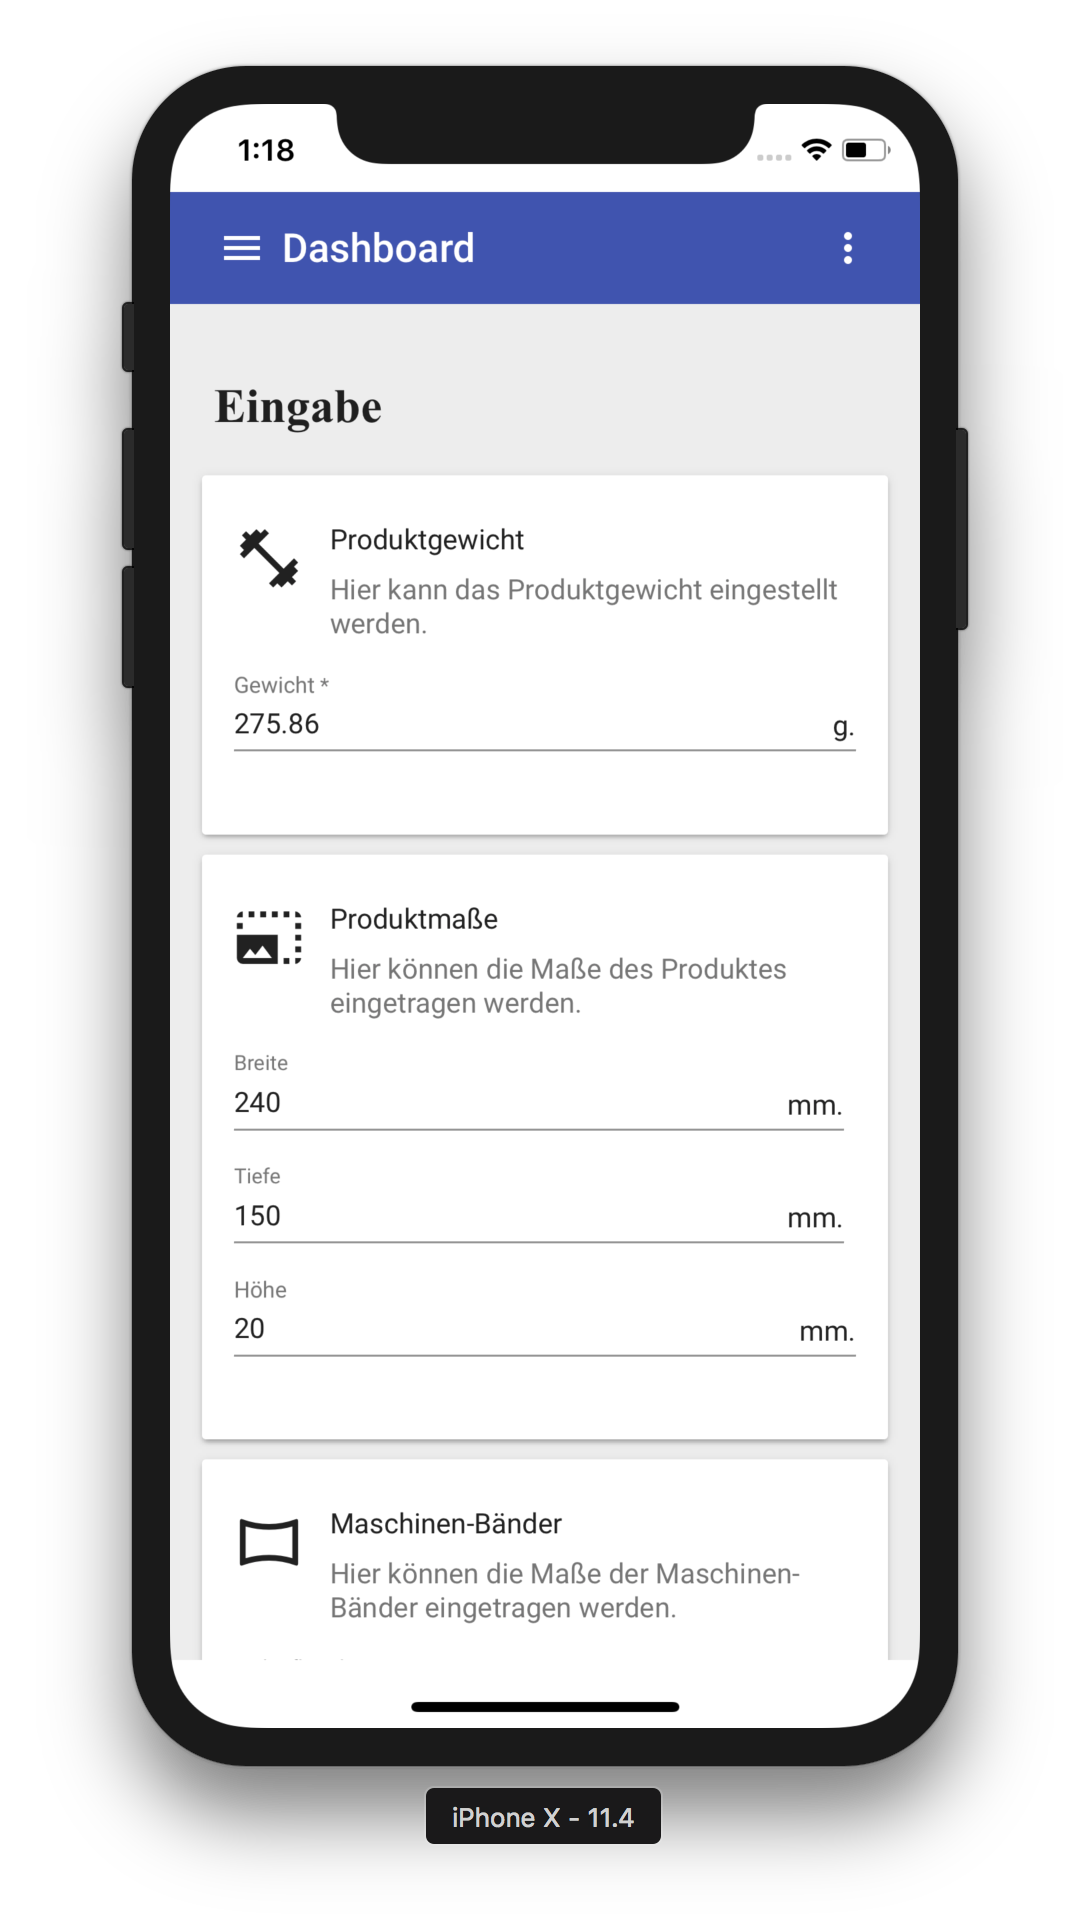
\includegraphics[scale=0.4]{images/kapitel_4/ios_app.png}
    \caption{iOS-App im Smartphone-Emulator}
    \label{fig:umsetzung_ios_app}
\end{figure}